\documentclass[10pt,a4paper]{article}

\usepackage[top=1.5cm, bottom=1.5cm, left=1.8cm, right=1.8cm]{geometry}
\usepackage{parskip}
\usepackage{titlesec}
\usepackage{enumitem}
\usepackage{multicol}
\usepackage{xcolor}
\usepackage{hyperref}
\usepackage[protrusion=false,expansion=false]{microtype}
\usepackage{tikz}
\usetikzlibrary{arrows.meta, positioning, backgrounds, fit}

% ── Colour palette ────────────────────────────────────────────────────────────
\definecolor{accent}  {RGB}{15,118,110}
\definecolor{cteal}   {RGB}{15,118,110}
\definecolor{cblue}   {RGB}{37, 99,235}
\definecolor{cpurple} {RGB}{124,58,237}
\definecolor{corange} {RGB}{194,65, 12}
\definecolor{cgreen}  {RGB}{5,150,105}
\definecolor{cgray}   {RGB}{75, 85, 99}

\hypersetup{colorlinks=true, urlcolor=accent, linkcolor=accent, pdfborder={0 0 0}}

% ── Section headings ─────────────────────────────────────────────────────────
\titleformat{\section}{\normalsize\bfseries\color{accent}}{}{0em}{}[\titlerule]
\titleformat{\subsection}{\small\bfseries}{}{0em}{}
\titlespacing{\section}   {0pt}{5pt}{2pt}
\titlespacing{\subsection}{0pt}{3pt}{1pt}

% ── List spacing ─────────────────────────────────────────────────────────────
\setlist[itemize] {noitemsep, topsep=1pt, leftmargin=1.2em}
\setlist[enumerate]{noitemsep, topsep=1pt, leftmargin=1.2em}
\setlength{\columnsep}{1.5em}
\setlength{\parskip}{2pt}

% ── TikZ node styles ─────────────────────────────────────────────────────────
\tikzset{
  bb/.style={rectangle, rounded corners=2pt,
             draw=#1!65!black, fill=#1!10,
             font=\tiny\bfseries, align=center,
             minimum height=0.48cm, inner xsep=4pt, inner ysep=2pt},
  arr/.style={-{Stealth[length=3.5pt,width=2.5pt]}, semithick, color=gray!55},
  lbl/.style={font=\tiny\itshape\color{gray!75}, midway},
}

% ── Helpers ───────────────────────────────────────────────────────────────────
\newcommand{\techfoot}{%
  \vspace{3pt}\rule{\linewidth}{0.4pt}\\
  {\footnotesize\color{gray!70}%
   \textbf{Stack:} Python\,3.13 · FastAPI · LangGraph · LangChain · ChromaDB ·
   FastMCP · Next.js\,16 · SQLite · Claude\,Sonnet\,4.6 / Ollama}%
}

% =============================================================================
\begin{document}

% ── Title ─────────────────────────────────────────────────────────────────────
\begin{center}
  {\large\bfseries Employee Onboarding AI Agent}\\[1.5pt]
  {\small\color{accent} Solution Design Document}
  \hspace{1em}{\footnotesize\color{gray!60}Acme Corp · April 2026}
\end{center}
\vspace{-2pt}\rule{\linewidth}{0.8pt}\vspace{3pt}

% =============================================================================
% DIAGRAM 1 — System Architecture (full width)
% =============================================================================
\begin{center}
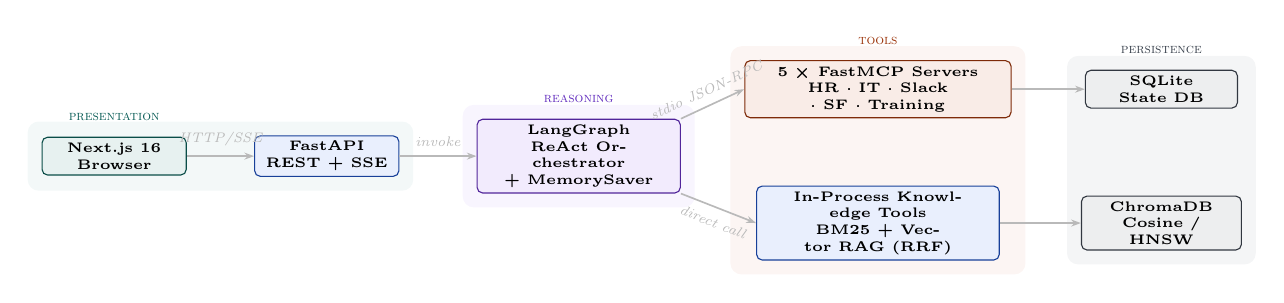
\begin{tikzpicture}
  % ── Nodes ──────────────────────────────────────────────────────────────────
  \node[bb=cteal,   text width=1.55cm] at (0,   0)    (fe)     {Next.js 16\\Browser};
  \node[bb=cblue,   text width=1.55cm] at (2.7, 0)    (api)    {FastAPI\\REST + SSE};
  \node[bb=cpurple, text width=2.3cm]  at (5.9, 0)    (agent)  {LangGraph\\ReAct Orchestrator\\+ MemorySaver};
  \node[bb=corange, text width=3.1cm]  at (9.7, 0.85) (mcp)    {5 × FastMCP Servers\\HR · IT · Slack · SF · Training};
  \node[bb=cblue,   text width=2.8cm]  at (9.7,-0.85) (rag)    {In-Process Knowledge Tools\\BM25 + Vector RAG (RRF)};
  \node[bb=cgray,   text width=1.65cm] at (13.3, 0.85)(sqlite) {SQLite\\State DB};
  \node[bb=cgray,   text width=1.75cm] at (13.3,-0.85)(chroma) {ChromaDB\\Cosine / HNSW};

  % ── Arrows ─────────────────────────────────────────────────────────────────
  \draw[arr] (fe)    -- node[lbl, above] {HTTP/SSE}    (api);
  \draw[arr] (api)   -- node[lbl, above] {invoke}      (agent);
  \draw[arr] (agent.north east) -- node[lbl, above, sloped] {stdio JSON-RPC} (mcp.west);
  \draw[arr] (agent.south east) -- node[lbl, below, sloped] {direct call}    (rag.west);
  \draw[arr] (mcp)   -- (sqlite);
  \draw[arr] (rag)   -- (chroma);

  % ── Layer background bands ─────────────────────────────────────────────────
  \begin{scope}[on background layer]
    \node[rounded corners=4pt, fill=cteal!5, inner sep=5pt,
          fit=(fe)(api)] {};
    \node[rounded corners=4pt, fill=cpurple!5, inner sep=5pt,
          fit=(agent)] {};
    \node[rounded corners=4pt, fill=corange!5, inner sep=5pt,
          fit=(mcp)(rag)] {};
    \node[rounded corners=4pt, fill=cgray!6, inner sep=5pt,
          fit=(sqlite)(chroma)] {};
  \end{scope}

  % ── Layer labels ───────────────────────────────────────────────────────────
  \node[font=\tiny\color{cteal!80!black},   above=0.08cm of fe]     {\textsc{presentation}};
  \node[font=\tiny\color{cpurple!80!black}, above=0.08cm of agent]  {\textsc{reasoning}};
  \node[font=\tiny\color{corange!80!black}, above=0.08cm of mcp]    {\textsc{tools}};
  \node[font=\tiny\color{cgray!80!black},   above=0.08cm of sqlite] {\textsc{persistence}};
\end{tikzpicture}
\end{center}

\vspace{3pt}
% =============================================================================
% Two-column body
% =============================================================================
\begin{multicols}{2}

\section{Architecture}

The diagram above shows the four layers. The browser communicates with a FastAPI backend that streams responses as Server-Sent Events (SSE). A LangGraph \texttt{create\_react\_agent} with \texttt{MemorySaver} is the reasoning core. It dispatches work to five FastMCP subprocess servers (simulating enterprise systems) via stdin/stdout JSON-RPC, and to in-process LangChain knowledge tools backed by ChromaDB. All structured state (employees, tickets, approvals) lives in SQLite.

\section{AI Agent Application}

The agent operates in a \textit{Reason → Act → Observe} loop, selecting tools based on the new hire's \texttt{role}, \texttt{level}, and \texttt{department}:

\begin{itemize}
  \item \textbf{Profile enrichment} — updates the HR record; provisions Salesforce and Slack accounts with role-specific fields.
  \item \textbf{Action execution} — opens IT tickets for hardware/software; assigns mandatory training modules matched to seniority.
  \item \textbf{Policy Q\&A} — answers freeform questions by retrieving semantically relevant chunks from the knowledge base with source attribution.
  \item \textbf{Approval workflows} — creates and tracks approval requests in-conversation.
  \item \textbf{Error handling} — each tool wraps calls in try/except and returns structured error strings; the agent re-plans without crashing.
\end{itemize}

\subsection{RAG Pipeline (3 production techniques)}
\begin{enumerate}
  \item \textbf{Cosine similarity} — ChromaDB collection configured with \texttt{hnsw:space=cosine} so relevance is magnitude-independent.
  \item \textbf{Contextual chunking} — each chunk is prefixed with its document title and section header before embedding, preserving meaning in isolation.
  \item \textbf{Hybrid retrieval} — BM25 keyword search and vector semantic search merged via Reciprocal Rank Fusion (equal 0.5/0.5 weighting with \texttt{EnsembleRetriever}).
\end{enumerate}

\section{Orchestration}

\textbf{Request flow:} User sends \texttt{POST /api/chat/\{id\}} → FastAPI hands off to the LangGraph orchestrator → agent issues tool calls (MCP servers or RAG) → results are observed and used for the next reasoning step → final text is streamed back as SSE and rendered as markdown in the browser.

\textbf{MCP communication:} Each of the five servers is a subprocess spawned at startup. \texttt{langchain-mcp-adapters} serialises tool calls to JSON-RPC over stdin/stdout, making them indistinguishable from native LangChain tools to the agent.

\textbf{Memory:} \texttt{MemorySaver} keeps per-employee conversation history keyed by \texttt{thread\_id}, enabling multi-turn context without re-querying the database each turn.

\section{Trade-offs \& Considerations}

\subsection{Assumptions \& Trade-offs}
\begin{itemize}
  \item \textbf{In-process RAG} — ChromaDB's embedded SQLite is unsafe for cross-process access on Windows. Knowledge tools run in the main process, sacrificing isolation to avoid file-lock deadlocks.
  \item \textbf{SQLite} — appropriate for development; production requires PostgreSQL with connection pooling.
  \item \textbf{Mock MCP servers} — simulate Workday, ServiceNow, Slack, Salesforce, and an LMS. Production integration needs OAuth, rate limiting, and idempotency guards.
  \item \textbf{In-RAM checkpointer} — \texttt{MemorySaver} is single-process only; multi-instance deployments need \texttt{PostgresSaver} or a Redis-backed checkpointer.
\end{itemize}

\subsection{Scalability}
The FastAPI layer is stateless per request. Horizontal scaling requires an external checkpointer. The BM25 index rebuilds at startup — fine for a static knowledge corpus; a dynamic knowledge base needs incremental indexing. ChromaDB should be replaced by a managed vector store (Pinecone, Weaviate, or PostgreSQL \texttt{pgvector}) at production scale.

\subsection{Security \& Governance}
\begin{itemize}
  \item All responses are scoped to the requesting \texttt{employee\_id}.
  \item Sensitive fields (salary, SSN) should be excluded via field-level access control before reaching LLM context.
  \item All tool invocations are audit-logged via \texttt{structlog}; these should be shipped to a SIEM.
  \item The \texttt{POST /api/admin/reset-db} endpoint must be gated by RBAC before deployment.
  \item The Ollama path (self-hosted models) satisfies data-residency and air-gapped deployment requirements.
\end{itemize}

\end{multicols}

% =============================================================================
% DIAGRAM 2 — Multi-Agent Topology (full width)
% =============================================================================
\newpage
\vspace{2pt}
\noindent{\normalsize\bfseries\color{accent}Multi-Agent Collaboration via MCP}
\vspace{2pt}
\rule{\linewidth}{0.5pt}
\vspace{3pt}

\begin{center}
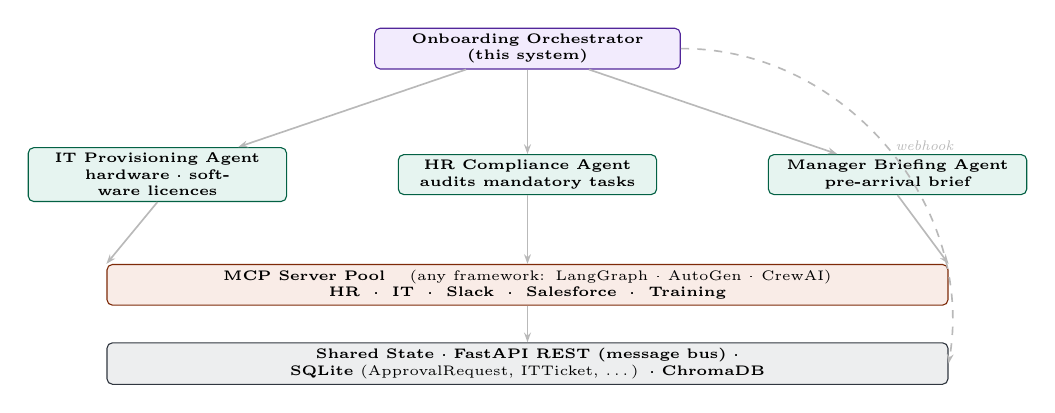
\begin{tikzpicture}
  % ── Orchestrator ───────────────────────────────────────────────────────────
  \node[bb=cpurple, text width=3.6cm] at (7, 3.0) (orch)
      {Onboarding Orchestrator\\(this system)};

  % ── Specialist agents ──────────────────────────────────────────────────────
  \node[bb=cgreen, text width=3.0cm] at (2.3, 1.4) (it)
      {IT Provisioning Agent\\hardware · software licences};
  \node[bb=cgreen, text width=3.0cm] at (7.0, 1.4) (hr)
      {HR Compliance Agent\\audits mandatory tasks};
  \node[bb=cgreen, text width=3.0cm] at (11.7,1.4) (mgr)
      {Manager Briefing Agent\\pre-arrival brief};

  % ── MCP pool ───────────────────────────────────────────────────────────────
  \node[bb=corange, text width=10.4cm] at (7.0, 0.0) (pool)
      {MCP Server Pool \hspace{0.5em}
       \textmd{(any framework: LangGraph · AutoGen · CrewAI)}\\
       HR \hspace{0.3em}·\hspace{0.3em} IT \hspace{0.3em}·\hspace{0.3em} Slack
       \hspace{0.3em}·\hspace{0.3em} Salesforce
       \hspace{0.3em}·\hspace{0.3em} Training};

  % ── Shared state ───────────────────────────────────────────────────────────
  \node[bb=cgray, text width=10.4cm] at (7.0,-1.0) (shared)
      {Shared State · FastAPI REST (message bus) ·
       SQLite \textmd{(ApprovalRequest, ITTicket, \ldots)} · ChromaDB};

  % ── Arrows ─────────────────────────────────────────────────────────────────
  \draw[arr] (orch) -- (it);
  \draw[arr] (orch) -- (hr);
  \draw[arr] (orch) -- (mgr);
  \draw[arr] (it.south)   -- (pool.north west);
  \draw[arr] (hr.south)   -- (pool.north);
  \draw[arr] (mgr.south)  -- (pool.north east);
  \draw[arr] (pool)       -- (shared);
  \draw[arr, dashed, bend left=50] (orch.east)
      to node[lbl, right] {webhook} (shared.east);
\end{tikzpicture}
\end{center}

\noindent{\footnotesize Because each MCP server exposes a standard JSON-RPC interface, any agent framework can attach to the same tool pool without modification. Agents coordinate through shared SQLite state and FastAPI REST endpoints, which act as a neutral message bus. The orchestrator can delegate sub-tasks to specialist agents and receive completion signals via webhook callbacks.}

\vspace{4pt}
\techfoot

\end{document}
